\subsection{Celle elettrolitiche}
Finora abbiamo visto reazioni chimiche che generano energia elettrica. Facciamo il contrario: prendiamoo una soluzione, immergiamo due elettrodi e applichiamo una d.d.p. dall'esterno.

Ciò che stiamo facendo è l'opposto di ciò che viene nelle pile. In esse infatti sfruttiamo reazioni chimiche per generare energia eletrrica, qui invece imponismo una una d.d.p. esterna e vogliamo vedere se avvengono reazioni chimiche. Tali reazioni dovranno avvenire, perché se avessimo elettroni sull'elettrodo e ioni positivi in soluzione, quest'ultimi tenderanno a depositarsi sull'elettrodo, catturando gli elettroni e quindi riducendosi. Se però su un elettrodo si ha riduzione, sull'altro dovrà avvenire un'ossidazione perché il circuito deve essere chiuso, altrimenti non fluirebbero gli elettroni da un elettrodo all'altro.

Consideriamo allora una soluzione di HCl in cui immergiamo due fili di platino e applichiamo una piccola d.d.p. che va via via aumentando. Man mano che sale riportiamo su un grafico i valori di intensità di corrente misurata e la d.d.p. appicata dall'esterno. Ci si accorge che se abbiamo un filo metallico, all'aumentare della d.d.p. aumenta anche la corrente che passa sul filo, mentre se abbiamo una soluzione ciò non accade.

Se adoperiamo un amperometro avente prontezza elavata, il quale misura immediatamente le più piccole variazioni di corrente, ci accorgiamo che la corrente ha un picco e poi ritorna a zero. Man mano che la d.d.p. aumenta avremo diversi picchi, fin quando questa non raggiunge un certo valore. Se invece non avessimo uno strumento abbastanza pronto vedremmo una corrente di fondo che poi invece cresce bruscamente:

\begin{figure}[H]
    \centering
    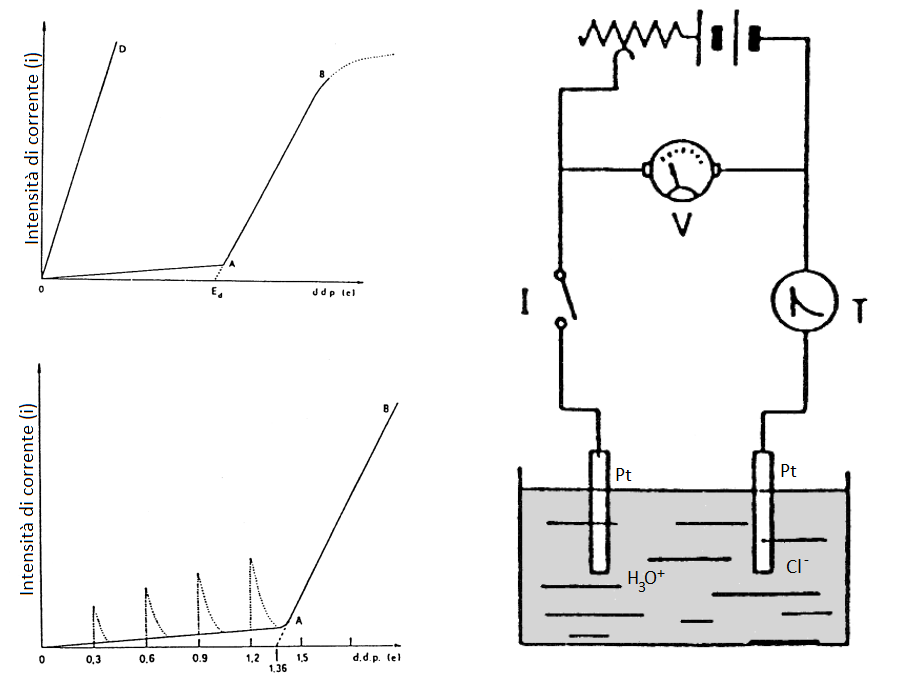
\includegraphics[width=14cm]{immagini/elettrolisi.png}
\end{figure}

A cosa è dovuto questo fenomeno?

In soluzione abbiamo HCl. Stiamo mettendo due fili di platino, che è un metallo nobile, inerte. Se applichiamo una d.d.p. ci aspettiamo che lo ione $\rm H_3O^+$ acquisti due elettroni e diventi $\rm H_2$, cioè si riduca, e questi due elettroni vengono forniti da due ioni $\rm Cl^-$ che diventano $\rm Cl_2$. Quindi il cloro si ossida perché perde due elettroni (uno per atomo), l'idrogeno si riduce perché acquista questi due elettroni.

Ci aspettiamo quindi che da HCl si formi $\rm H_2$ al catodo (le riduzioni avvengono sempre al catodo) e $\rm Cl_2$ all'anodo. Se però questo fenomeno avviene significa che c'è uno scambio di elettroni, quindi dobbiamo vedere crescere l'intensità di corrente. Noi però vediamo che cresce per poi tornare a zero ripetutamente. Perché?

Ciò che succede è che la reazione avviene, ma nell'istante in cui si sviluppano le prime bollicine di $\rm H_2$ queste resteranno aderite al catodo che è costituito da un filo di platino. Inoltre nell'istante in cui si sviluppano le prime bollicine di $\rm Cl_2$ esse resteranno aderite all'anodo. In questo modo essere trasformano gli elettrodi in platino in elettrodo a idrogeno e elettrodo al cloro. Questi due elettrodi accoppiati formano una pila che genera una d.d.p. chiamata \textbf{forza contro-elettromotrice}, in opposizione alla d.d.p. esterna. Quindi la pila (nel caso particolare della pila cloro-idrogeno) che si è formata a causa delle speci che si legano agli elettrodi genera una d.d.p. che ha segno opposto a quella che applichiamo, per cui il passaggio di corrente crolla.

Nota: la pila si è generata all'interno della cella elettrolitica.

Non vedendo passare corrente, aumentiamo la d.d.p. applicata. La reazione ripartirà, generando altro gas $\rm H_2$ e altro gas $\rm Cl_2$, quindi rispetto alla pila la loro attività aumenterà e dunque riaumenterà la $f_{c.e.m.}$, bloccando di nuovo la reazione. Continuando ad aumentare la d.d.p. esterna tale fenomeno si ripete, fino a quando la pressione dei gas che si stanno depositando sugli elettrodi raggiunge la pressione atmosferica. A quel punto non se ne potrà accumulare più: il gas successivo dovrà fuoriuscire perché supera la pressione atmosferica, quindi la $f_{c.e.m.}$ non aumenta più in quanto la concentrazione di cloro e idrogeno agli elettrodi non aumenta più avendo raggiunto il limite massimo che è 1 atm (non possiamo avere concentrazioni di gas superiore a 1 atm in un ambiente ad 1 atm). %ah??? concentrazioni in atm?

Nel momento in cui vediamo i due gas fuoriuscire vuol dire che abbiamo fatto elettrolisi.

Va da notare che con un filo metallico non è necessario superare una soglia, ma d'altro le soluzioni conducono per la presenza di ioni (conduttori di seconda specie).

Il potenziale di soglia è specifico per ogni reazione. Al di sopra di esso avviene l'elettrolisi. Al di sotto no.

\begin{equation*}
    \left.\begin{aligned}
    \text{Catodo} \; (-) \quad \ce{2H_3O^+ + 2e^- -> 2H_2O + H_2 ^}\\
    \text{Anodo} \; (+) \hspace{1.9cm} \quad \ce{2Cl^- -> Cl_2 ^ + 2 e^-}
  \end{aligned}\right\} f_{c.e.m.}=1.36 V
\end{equation*}

Quindi se vogliamo elettrolizzare un metallo abbiamo un valore che è quello termodinamico, il quale deve essere superato per far sì che il fenomeno avvenga con efficienza. Ad esempio in questo caso se non superiamo 1.36 V non elettrolizzeremo mai l'acido cloridrico, e nemmeno se applichiamo proprio quel valore: dobbiamo applicarne di più. 

La tensione in più da applicare si chiama \textbf{sovratensione}. Essa si applica affinché il fenomeno avvenga in modo efficiente.

Per gli elementi che nella tabella dei potenziali stanno appena sopra l'idrogeno, se usiamo un filo di platino (perché dipende dall'elettrodo) la sovratensione da applicare è parecchia, circa 0.7V.

Quindi, nonostante da un punto di vista termodinamico sembri impossibile, possiamo comunque ridurre i primi elementi sopra l'idrogeno, in quanto quest'ultimo su un elettrodo di platino si riduce solo se applichiamo una sovratensione di 0.6 V.

Continua però a valere la regola che se abbiamo più di una specie in soluzione, si ridurrà quella che ha un potenziale di riduzione maggiore.

\subsection{Elettrolisi di sali fusi}

Se avessimo delle soluzioni acquose di $\rm MgCl_2$ o NaCl, non potremmo avere la riduzione degli ioni metallici $\rm Na^+$ in Na e $\rm Mg^{2+}$ in Mg, in quanto in acqua è presente lo ione $\rm H_3O^+$ che, avendo potenziale di riduzione maggiore, è la specie che si riduce.

I sali fusi possono però essere ridotti anche in assenza di acqua.

Per far ridurre l'NaCl lo mettiamo in un crogiolo di ossido di alluminio $\rm Al_2O_3$ (che può arrivare fino a 3000 gradi), riscaldiamo fino a 800° C cosicché l'NaCl fonde. Immergiamo gli elettrodi nel fuso e elettrolizziamo l'NaCl

\begin{figure}[H]
    \centering
    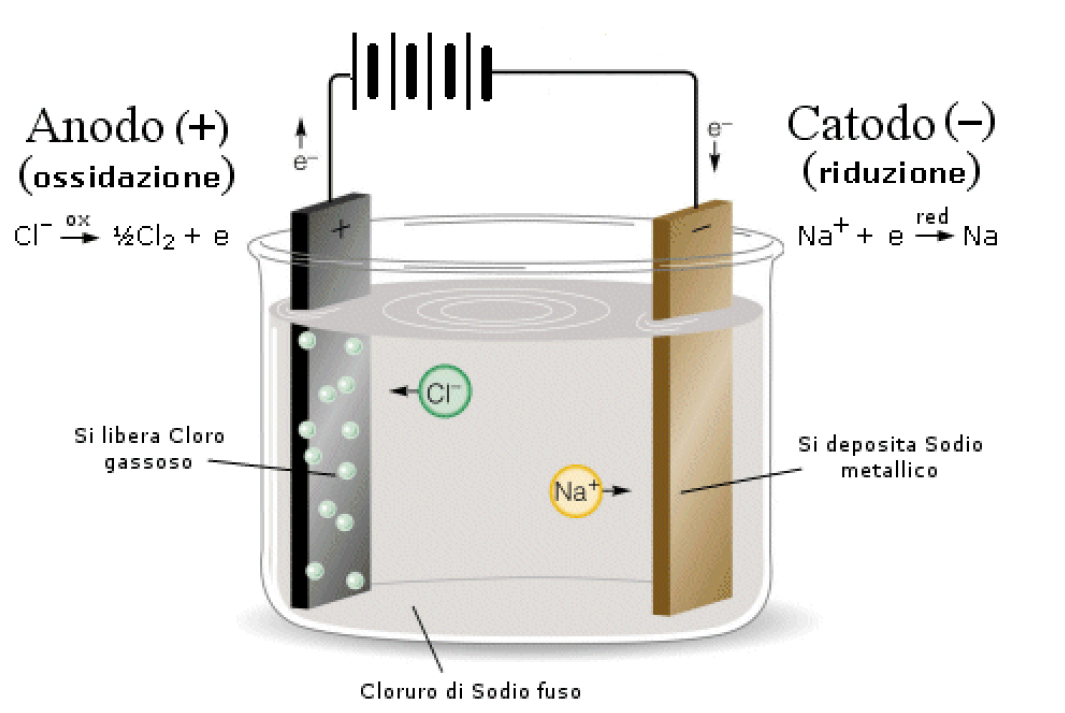
\includegraphics[width=12cm]{immagini/elettrolisi_sali_fusi.png}
\end{figure}

\begin{center}
    \begin{tabular}{p{7.8cm}}
        \hspace{-0.6cm}$\begin{cases}
        \ce{2Cl^- -> Cl_2 ^ + 2e^-}\\
        \ce{2H_3O^+ + 2e^- -> 2H_2O + H_2 ^}
        \end{cases}$\\
        \\[-1.5ex]
        \hline
        \\[-1.5ex]
        \hspace{-0.2cm}\ce{2Cl^- +2H_3O^+ -> Cl_2 ^ + H_2 ^ + 2H_2O}
    \end{tabular}
\end{center}

\subsection{Accumulatore al piombo (batteria automobile)}

\begin{figure}[H]
    \centering
    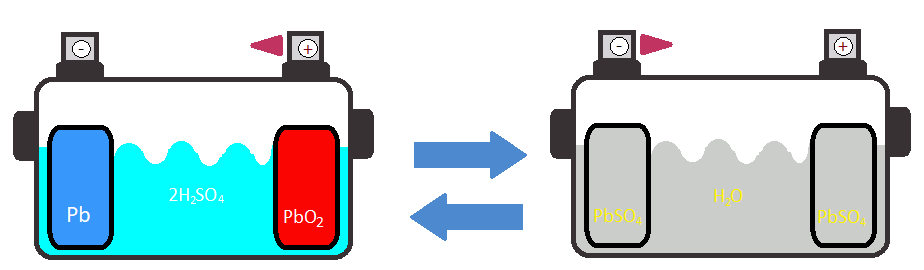
\includegraphics[width=15cm]{immagini/accumulatore_al_piombo.png}
\end{figure}

Abbiamo l'anodo costituito da piombo metallico e il catodo da $\rm PbO_2$ (quindi $\rm Pb^{4+}$). La soluzione che ci permette di trasportare gli elettrodi è acido solforico $\rm H_2SO_4$ molto concentrato, al 30\%, tant'è che quando si abbassa il livello del liquido nella batteria non si aggiunge acido ma acqua, in quanto l'$\rm H_2SO_4$ bolle a 400° C, per cui se il livello si è abbassato sarà evaporata soltanto l'acqua.

Durante la fase di scarica ciò che succede è che il $\rm Pb^0(s)$ in presenza di acido solforico (e quindi di ioni solfato $\rm SO_4^{2-}$) libera 2 elettroni, diventando $\rm Pb^{2+}$. Si unisce quindi allo ione solfato dando $\rm PbSO_4$ e liberando 2 elettroni.

$$(-)\; \ce{Pb(s) + SO_4^{2-} -> PbSO_4(s) + 2e^-}$$

Questi due elettroni vengono catturati dal $\rm PbO_2(s)$, e il piombo passa da $\rm Pb^{4+}$ a $\rm Pb^{2+}$, per poi unirsi allo ione solfato e diventare $\rm PbSO_4$:

$$(+)\; \ce{PbO_2(s) + 4H_3O^+ + SO_4^{2-} +2e^- -> PbSO_4(s) + 6H_2O}$$

Quindi in entrambi i casi si forma $\rm PbSO_4$, però una volta a partire da $\rm Pb^0$ che deve liberare 2 elettroni e una volta a partire da $\rm Pb^{4+}$ che deve acquistare 2 elettroni.

Nel proceso di carica invece avviene l'opposto: abbiamo $\rm PbSO_4$ (quindi $\rm Pb^{2+}$) che nell'anodo assorbe 2 elettroni diventando Pb(s) mentre nel catodo cede 2 elettroni diventando $\rm Pb^{4+}$:

$$(-) \; \ce{PbSO_4(s) + 2e^- -> Pb(s) + SO_4^{2-}}$$

$$(+) \; \ce{PbSO_4(s) + 6H_2O  -> PbO_2(s) + 4H_3O^+ + SO_4^{2-} +2e^-}$$

La reazione che avviene globalmente è

$$\ce{Pb + PbO_2 + 2H_2SO_4 <--> 2PbSO_4 + 2H}$$

Il piombo col biossido di piombo in acido solforico diventano $\rm PbSO_4$. La reazione va in entrambe le direzioni,

Caloliamo la $f.e.m.$\,:

\begin{center}
    \begin{tabular}{p{8.8cm}}
        \hspace{-0.6cm}$\begin{cases}
        \ce{Pb(s) + SO_4^{2-} -> PbSO_4 + 2e^-}, \; E_0=-0.36V\\
        \ce{ClO^- + 4OH^- -> PbSO_4(s) + 6H_2O}, \; E_0= 1.69 V
        \end{cases}$\\
        \\[-1.5ex]
        \hline
        \\[-1.5ex]
        \hspace{-0.2cm}\ce{3ClO^- -> 2Cl^- + ClO_3^-}
    \end{tabular}
\end{center}

$$\implies E_0=1.69 - (-0.36)=2.04V$$

Ogni coppia di elettrodi dà questo potenziale, per cui se vogliamo una d.d.p. di 12 V come nelle batterie delle auto dobbiamo mettere 6 coppie in serie.
\subsection{Leggi di Faraday}
Il fenomeno dell'elettrolisi è generato dalle due leggi di Faraday.

\vspace{0.2cm}$\bullet$\textbf{Prima legge di Faraday}

\vspace{0.2cm}\textit{"La massa di una sostanza che si libera agli elettrodi è proporzionale alla quantità di elettricità passata attraverso la soluzione."}

\vspace{0.2cm}$\bullet$\textbf{Seconda legge di Faraday}

\vspace{0.2cm}\textit{"Al fine di liberare agli elettrodi 1 equivalente di una qualsiasi sostanza è necessario che attraverso la soluzione passino 96.485 C (quantità nota come Faraday). Naturalmente se attraverso la soluzione passano n Faraday verranno liberati n equivalenti."}

\vspace{0.2cm}Il Faraday (F) è la quantità di elettricità portata da 1 mole di elettroni ( N elettroni).

Vediamo un esempio numerico:

\vspace{0.2cm}\textbf{EXR} Che intensità di corrente $I$ è necessaria affinché in 24 ore essa separi un kg di rame Cu da una soluzione a partire da $\rm Cu^{2+}$?

\vspace{0.2cm}\textbf{SOL:} La reazione che deve avvenire è

$$\ce{Cu^{2+} + 2e^- -> Cu^0}$$

Per le leggi di Faraday la quantità di sostanza depositata agli elettrodi è proporzionale ai Faraday di corrente passati. In particolare 1 Faraday di corrente deposita sempre 1 equivalente, e ciò per qualsiasi sostanza. 1 Faraday equivale a 96485 C.

La carica $Q$ è pari a

$$Q=I \cdot t(s)$$

Vediamo quanti equivalenti ci sono in un kg di rame. Il peso atomico del rame è 63.546, ma siccome stiamo scambiando due elettroni il peso equivalente sarà diviso 2, cioè 31.773. Peranto in un kg di rame avremo

$$\frac{1000}{31.773} = 31.4733 \; \text{equivalenti}$$

Per depositarli saranno necessari 31.4733 F di corrente, cioè $31.4733 \cdot 96485 = 3036701.351 \, C$. Questa carica, divisa per il tempo espresso in secondi, darà l'intensità di corrente necessaria:

$$\frac{Q}{t(s)} = I = \frac{3036701.351}{24 \cdot 3600} = 35.147 \; \text{Ampere}$$